\section{Problem 1: FFT of Single Tone sinusoidal wave}

\begin{enumerate}
    \item The function generator was set to a sinusoidal wave with a $500$Hz frequency, 2$V_{pp}$ amplitude, and no offset. The measure function was used to verify all the properties of the signal, and a hardcopy was subsequently taken.
          \begin{figure}[H]
              \centering
              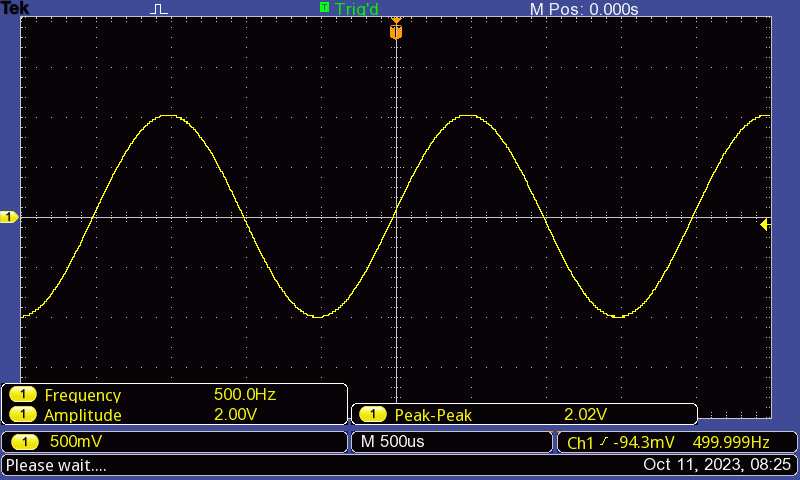
\includegraphics[width=0.8\linewidth]{images/problem1_hardcopy1.png}
              \caption{Hardcopy of the signal}
              \label{fig:problem1_hardcopy1}
          \end{figure}
    \item Afterward, the FFT spectrum was obtained via the spectrum's FFT function. The cursor was used to measure the properties of the spectrum, and then a hardcopy was taken. Furthermore, another hardcopy was taken of the zoomed in spectrum.
          \begin{figure}
              \centering
              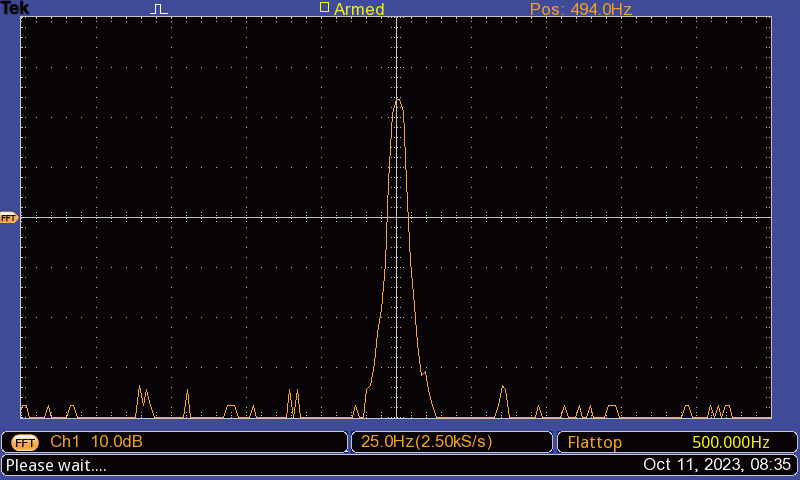
\includegraphics[width=0.5\linewidth]{images/problem1_hardcopy2.png}
              \caption{Hardcopy of the FFT spectrum, showing 494Hz.}
              \label{fig:problem1_hardcopy2}
          \end{figure}
          \begin{figure}[H]
              \centering
              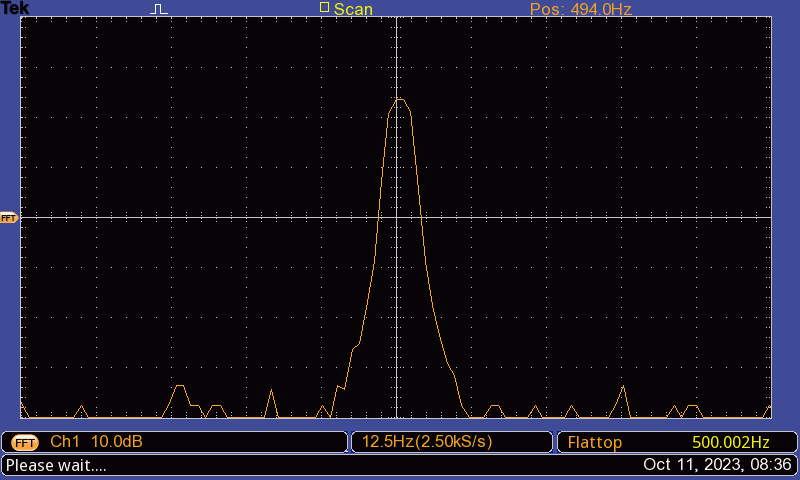
\includegraphics[width=0.5\linewidth]{images/problem1_hardcopy3.png}
              \caption{Hardcopy of the zoomed in FFT spectrum, showing 494Hz.}
              \label{fig:problem1_hardcopy3}
          \end{figure}
          What is immediately noticed, however, is that the position seems to show 494Hz. This is in fact an error of $1\%$, when the usual error should be around $0.1\%$. The reason this error shows up may be due to the miscalibration of the Oscilloscope.
    \item For the sinusoidal wave with a 2KHz frequency(without any offset) to have a 0dB spectrum peak, the $V_{pp}$ was found to be around 2.7$V_{pp}$. A hardcopy of the time-domain signal was taken.
          \begin{figure}[H]
              \centering
              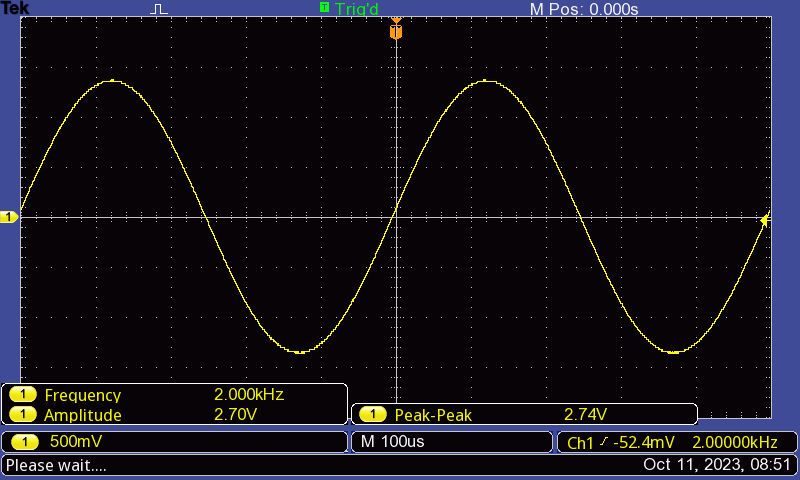
\includegraphics[width=0.75\linewidth]{images/problem1_hardcopy4.png}
              \caption{Hardcopy of the time-domain signal with 0dB spectrum peak.}
              \label{fig:problem1_hardcopy4}
          \end{figure}
          Then, a hardcopy is taken of the frequency spectrum that is obtained by using the FFT function on the oscilloscope.
          \begin{figure}[H]
              \centering
              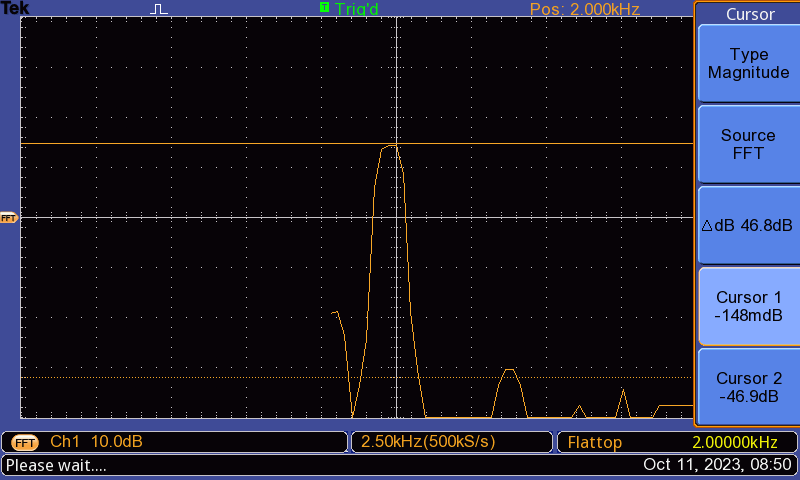
\includegraphics[width=0.75\linewidth]{images/problem1_hardcopy5.png}
              \caption{Hardcopy of the frequency spectrum with 0dB spectrum peak.}
              \label{fig:problem1_hardcopy5}
          \end{figure}
          It is observed that the cursor shows a dB of $-148$mdB which is close to $0$dB. The small error is because of the Oscilloscope's resolution. It also shows the 2KHz frequency.
\end{enumerate}

\section{Problem 2:}
\begin{enumerate}
    \item The function generator is used to generate a square wave at $2V_{pp}$ amplitude, a 1ms period, and no offset. A hardcopy of the signal is then taken.
          \begin{figure}[H]
              \centering
              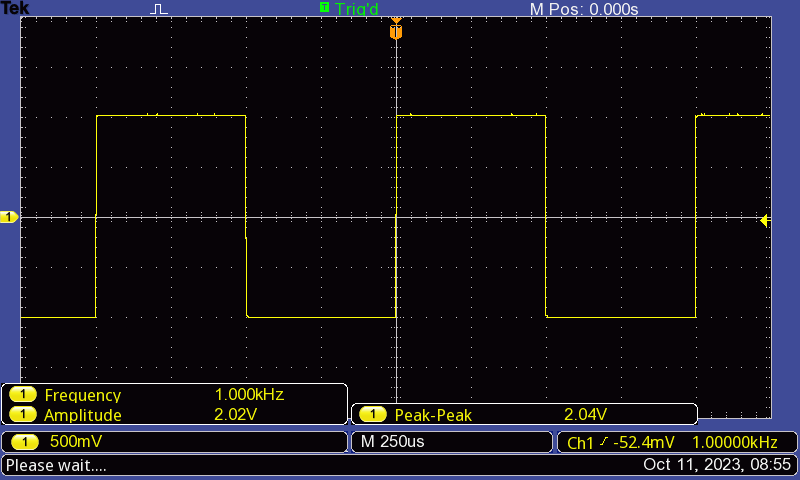
\includegraphics[width=0.75\linewidth]{images/problem2_hardcopy1.png}
              \caption{Hardcopy of the square wave signal.}
              \label{fig:problem2_hardcopy1}
          \end{figure}
    \item The FFT spectrum is then obtained, and zoomed into, subsequently hardcopies of each frequency component are taken. The harmonics observed are as follows:
          \begin{itemize}
              \item 1050Hz: -989mdB
              \item 2950Hz: -10.1dB
              \item 5000Hz: -14.9dB
              \item 7000Hz: -17.7dB
          \end{itemize}
          Hardcopies are taken of the cursor over each of the harmonics.
          \begin{figure}[H]
              \centering
              \begin{subfigure}{0.4\textwidth}
                  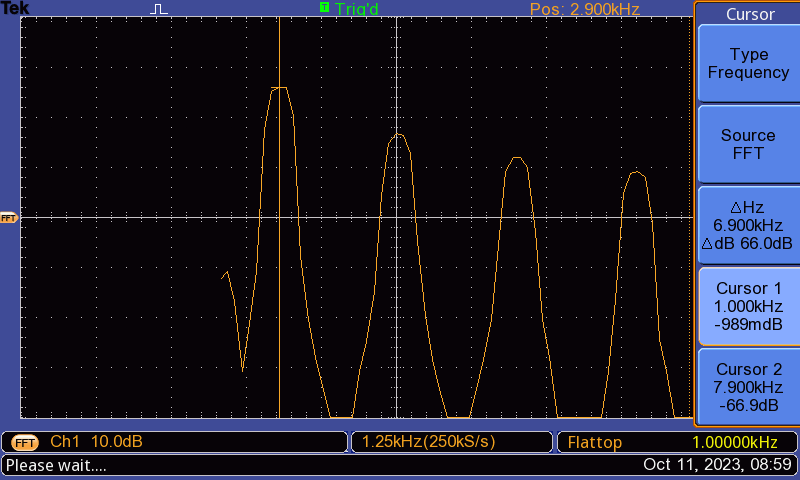
\includegraphics[width=\linewidth]{images/problem2_hardcopy2.png}
              \end{subfigure}
              \begin{subfigure}{0.4\textwidth}
                  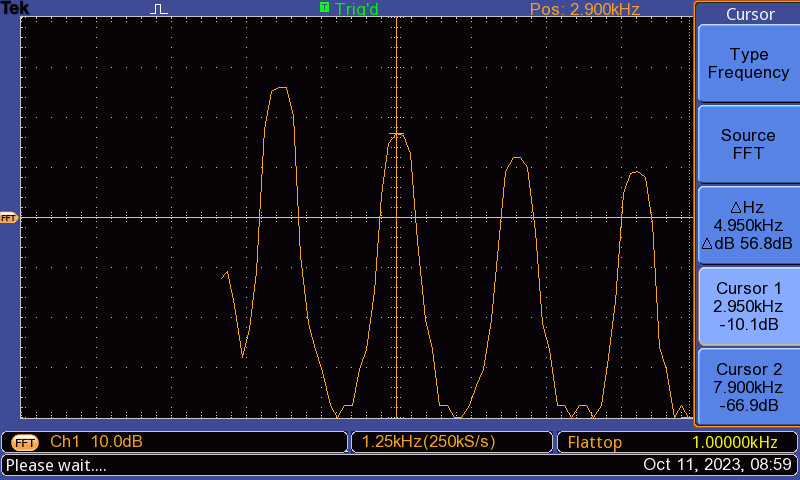
\includegraphics[width=\linewidth]{images/problem2_hardcopy3.png}
              \end{subfigure}
              \begin{subfigure}{0.4\textwidth}
                  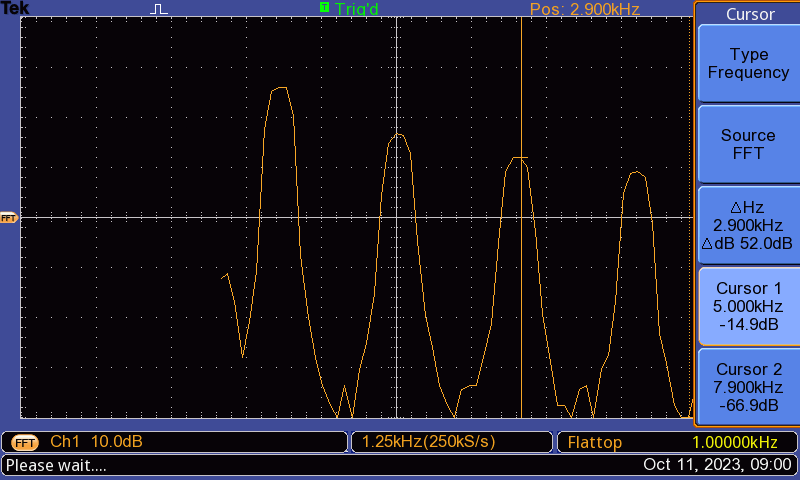
\includegraphics[width=\linewidth]{images/problem2_hardcopy4.png}
              \end{subfigure}
              \begin{subfigure}{0.4\textwidth}
                  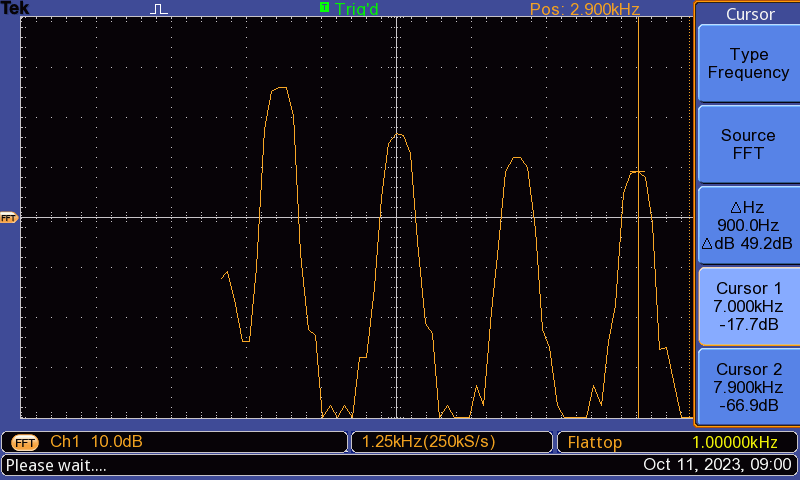
\includegraphics[width=\linewidth]{images/problem2_hardcopy5.png}
              \end{subfigure}
              \caption{The harmonics of the square wave.}
          \end{figure}
          Which are pretty consistent with theory and the square wave on the screen, in that the harmonics are odd multiples of the fundamental frequency.
    \item The FFT spectrum is then obtained for 20\% duty cycles, the amplitudes of the first four harmonics are measured and hardcopies are taken of the signal both in time and frequency domain.
          \begin{figure}[H]
              \centering
              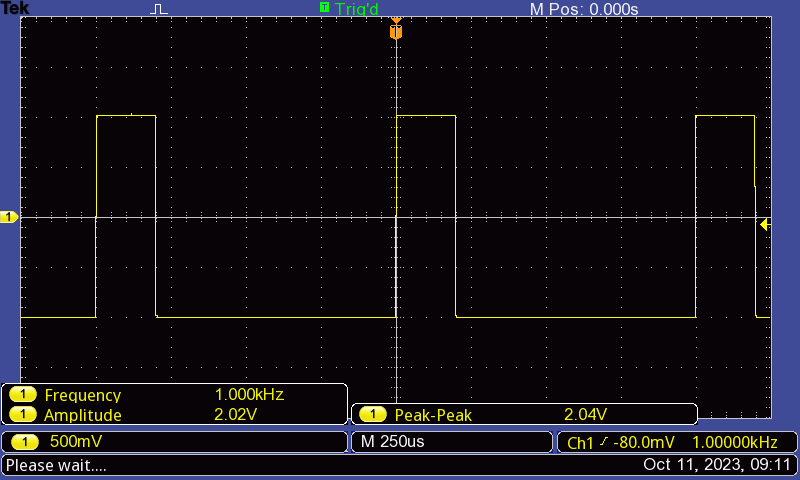
\includegraphics[width=0.75\linewidth]{images/problem2_hardcopy7.png}
              \caption{Hardcopy of the 20\% duty cycle square wave.}
              \label{fig:problem2_hardcopy6}
          \end{figure}
          \begin{figure}[H]
              \centering
              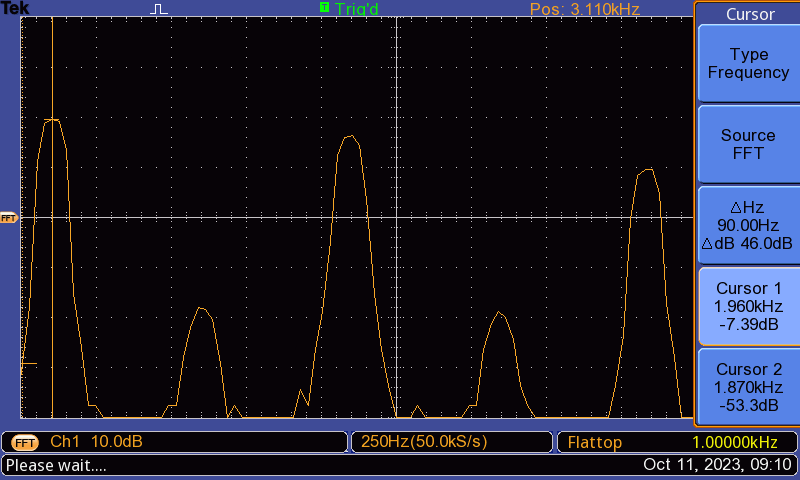
\includegraphics[width=0.75\linewidth]{images/problem2_hardcopy6.png}
              \caption{Hardcopy of the 20\% duty cycle square wave FFT spectrum.}
              \label{fig:problem2_hardcopy7}
          \end{figure}
          The harmonics were then taken by using the cursor, the following values were obtained for the non-DC harmonics:
          \begin{itemize}
              \item 1010Hz: -5.39dB
              \item 2010Hz: -7.39dB
              \item 2970Hz: -10.9dB
              \item 3980Hz: -17.3dB
          \end{itemize}
          Because the signal is at a 20\% duty cycle, the harmonics are no longer odd multiples of the fundamental frequency.
\end{enumerate}

\newpage
\section{Problem 3: FFT of Multiple-Tone sinusoidal wave}
The following circuit is assembled.
\begin{figure}[H]
    \centering
    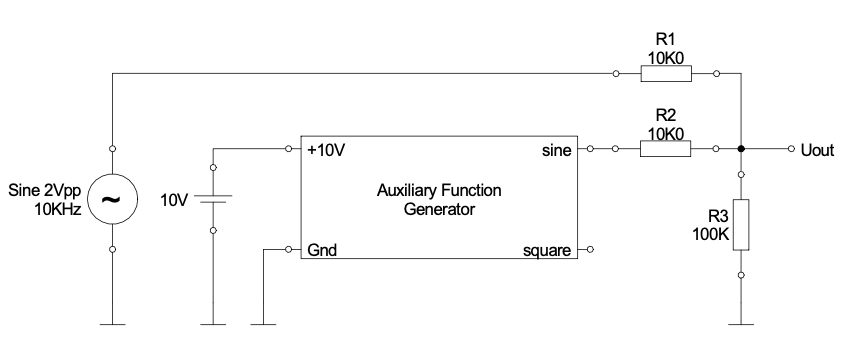
\includegraphics[width=0.75\linewidth]{images/problem3_circuit.png}
    \caption{The circuit used for problem 3.}
    \label{fig:problem3_circuit}
\end{figure}

Hardcopies of the signal and the signal's spectrum are then taken.
\begin{figure}[H]
    \centering
    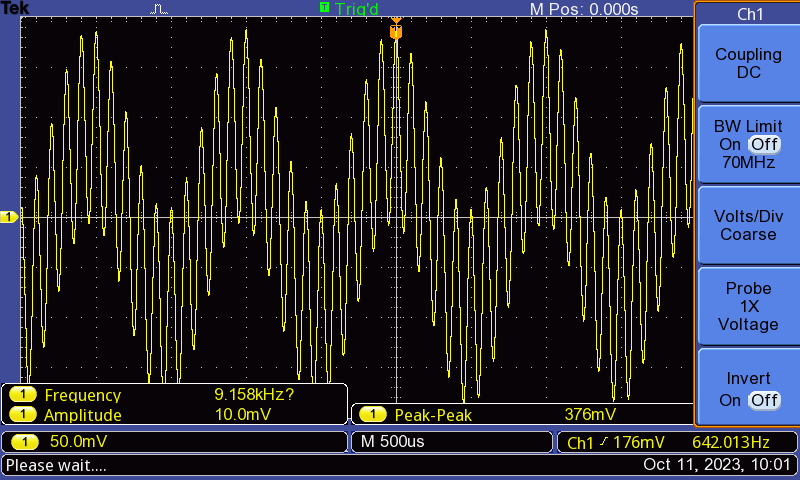
\includegraphics[width=0.85\linewidth]{images/problem3_hardcopy1.png}
    \caption{Hardcopy of the signal.}
    \label{fig:problem3_hardcopy1}
\end{figure}

\begin{figure}[H]
    \centering
    \begin{subfigure}{0.8\textwidth}
        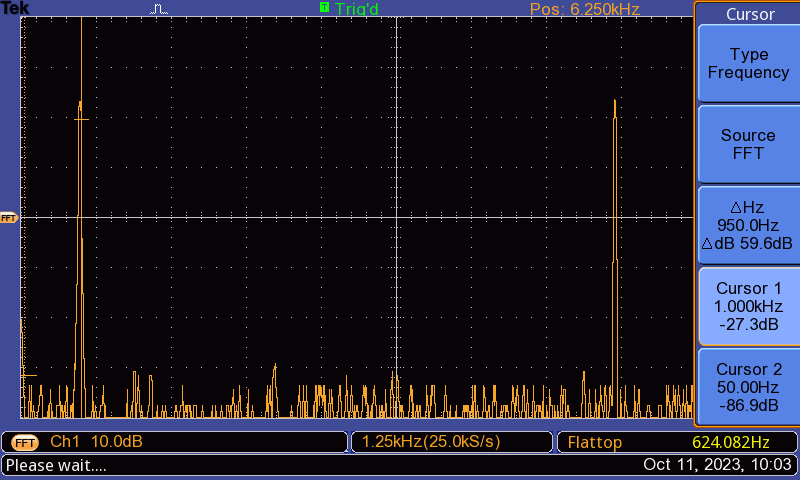
\includegraphics[width=\linewidth]{images/problem3_hardcopy2.png}
    \end{subfigure}
    \begin{subfigure}{0.8\textwidth}
        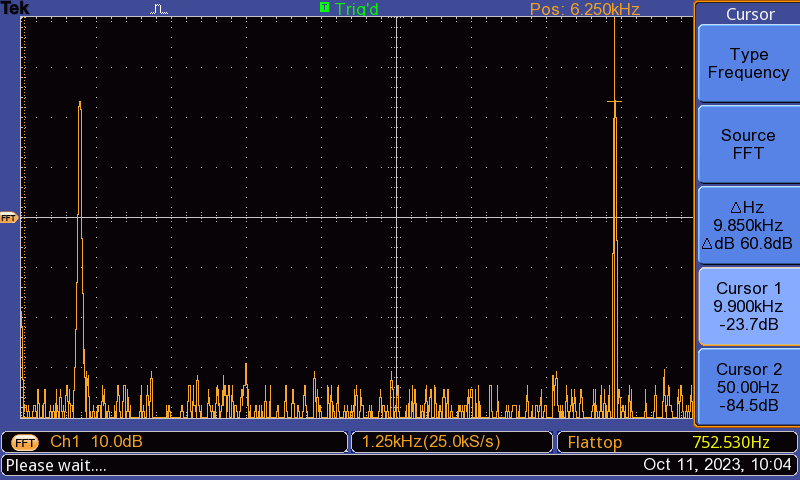
\includegraphics[width=\linewidth]{images/problem3_hardcopy3.png}
    \end{subfigure}
    \caption{\centering Hardcopy of the signal's spectrum, and the frequencies measured at 1000kHz and 9900kHz, respectively}
    \label{fig:problem3_hardcopy2}
\end{figure}